%-----------------------------------------------------------------------------------------------------------------------------------------------%
%	The MIT License (MIT)
%
%	Copyright (c) 2019 Jan Küster
%
%	Permission is hereby granted, free of charge, to any person obtaining a copy
%	of this software and associated documentation files (the "Software"), to deal
%	in the Software without restriction, including without limitation the rights
%	to use, copy, modify, merge, publish, distribute, sublicense, and/or sell
%	copies of the Software, and to permit persons to whom the Software is
%	furnished to do so, subject to the following conditions:
%	
%	THE SOFTWARE IS PROVIDED "AS IS", WITHOUT WARRANTY OF ANY KIND, EXPRESS OR
%	IMPLIED, INCLUDING BUT NOT LIMITED TO THE WARRANTIES OF MERCHANTABILITY,
%	FITNESS FOR A PARTICULAR PURPOSE AND NONINFRINGEMENT. IN NO EVENT SHALL THE
%	AUTHORS OR COPYRIGHT HOLDERS BE LIABLE FOR ANY CLAIM, DAMAGES OR OTHER
%	LIABILITY, WHETHER IN AN ACTION OF CONTRACT, TORT OR OTHERWISE, ARISING FROM,
%	OUT OF OR IN CONNECTION WITH THE SOFTWARE OR THE USE OR OTHER DEALINGS IN
%	THE SOFTWARE.
%	
%
%-----------------------------------------------------------------------------------------------------------------------------------------------%


%============================================================================%
%
%	DOCUMENT DEFINITION
%
%============================================================================%

%we use article class because we want to fully customize the page and don't use a cv template
\documentclass[10pt,A4]{article}	
\usepackage{lmodern}

%----------------------------------------------------------------------------------------
%	ENCODING
%----------------------------------------------------------------------------------------

% we use utf8 since we want to build from any machine
\usepackage[utf8]{inputenc}		

%----------------------------------------------------------------------------------------
%	LOGIC
%----------------------------------------------------------------------------------------

% provides \isempty test
\usepackage{xstring, xifthen}

%----------------------------------------------------------------------------------------
%	FONT BASICS
%----------------------------------------------------------------------------------------

% some tex-live fonts - choose your own

%\usepackage[defaultsans]{droidsans}
%\usepackage[default]{comfortaa}
%\usepackage{cmbright}
%\usepackage[default]{raleway}
%\usepackage{fetamont}
%\usepackage[default]{gillius}
\usepackage[light,math]{iwona}
%\usepackage[thin]{roboto} 

% set font default
\renewcommand*\familydefault{\sfdefault} 	
\usepackage[T1]{fontenc}

% more font size definitions
\usepackage{moresize}


%----------------------------------------------------------------------------------------
%	FONT AWESOME ICONS
%---------------------------------------------------------------------------------------- 

% include the fontawesome icon set
\usepackage{fontawesome}

% use to vertically center content
% credits to: http://tex.stackexchange.com/questions/7219/how-to-vertically-center-two-images-next-to-each-other
\newcommand{\vcenteredinclude}[1]{\begingroup
\setbox0=\hbox{\includegraphics{#1}}%
\parbox{\wd0}{\box0}\endgroup}

% use to vertically center content
% credits to: http://tex.stackexchange.com/questions/7219/how-to-vertically-center-two-images-next-to-each-other
\newcommand*{\vcenteredhbox}[1]{\begingroup
\setbox0=\hbox{#1}\parbox{\wd0}{\box0}\endgroup}

% icon shortcut
\newcommand{\icon}[3] { 							
	\makebox(#2, #2){\textcolor{maincol}{\csname fa#1\endcsname}}
}	

% icon with text shortcut
\newcommand{\icontext}[4]{ 						
	\vcenteredhbox{\icon{#1}{#2}{#3}}  \hspace{2pt}  \parbox{0.9\mpwidth}{\textcolor{#4}{#3}}
}

% icon with website url
\newcommand{\iconhref}[5]{ 						
    \vcenteredhbox{\icon{#1}{#2}{#5}}  \hspace{2pt} \href{#4}{\textcolor{#5}{#3}}
}

% icon with email link
\newcommand{\iconemail}[5]{ 						
    \vcenteredhbox{\icon{#1}{#2}{#5}}  \hspace{2pt} \href{mailto:#4}{\textcolor{#5}{#3}}
}

%----------------------------------------------------------------------------------------
%	PAGE LAYOUT  DEFINITIONS
%----------------------------------------------------------------------------------------

% page outer frames (debug-only)
% \usepackage{showframe}		

% we use paracol to display breakable two columns
\usepackage{paracol}

% define page styles using geometry
\usepackage[a4paper]{geometry}

% remove all possible margins
\geometry{top=1cm, bottom=1cm, left=1cm, right=1cm}

\usepackage{fancyhdr}
\pagestyle{empty}

% space between header and content
% \setlength{\headheight}{0pt}

% indentation is zero
\setlength{\parindent}{0mm}

%----------------------------------------------------------------------------------------
%	TABLE /ARRAY DEFINITIONS
%---------------------------------------------------------------------------------------- 

% extended aligning of tabular cells
\usepackage{array}

% custom column right-align with fixed width
% use like p{size} but via x{size}
\newcolumntype{x}[1]{%
>{\raggedleft\hspace{0pt}}p{#1}}%


%----------------------------------------------------------------------------------------
%	GRAPHICS DEFINITIONS
%---------------------------------------------------------------------------------------- 

%for header image
\usepackage{graphicx}

% use this for floating figures
% \usepackage{wrapfig}
% \usepackage{float}
% \floatstyle{boxed} 
% \restylefloat{figure}

%for drawing graphics		
\usepackage{tikz}				
\usetikzlibrary{shapes, backgrounds,mindmap, trees}

%----------------------------------------------------------------------------------------
%	Color DEFINITIONS
%---------------------------------------------------------------------------------------- 
\usepackage{transparent}
\usepackage{color}

% primary color
%\definecolor{maincol}{RGB}{ 225, 0, 0 }
\definecolor{maincol}{RGB}{0,113 188}

% accent color, secondary
% \definecolor{accentcol}{RGB}{ 250, 150, 10 }

% dark color
\definecolor{darkcol}{RGB}{ 70, 70, 70 }

% light color
\definecolor{lightcol}{RGB}{245,245,245}


% Package for links, must be the last package used
\usepackage[hidelinks]{hyperref}

% returns minipage width minus two times \fboxsep
% to keep padding included in width calculations
% can also be used for other boxes / environments
\newcommand{\mpwidth}{\linewidth-\fboxsep-\fboxsep}
	


%============================================================================%
%
%	CV COMMANDS
%
%============================================================================%

%----------------------------------------------------------------------------------------
%	 CV LIST
%----------------------------------------------------------------------------------------

% renders a standard latex list but abstracts away the environment definition (begin/end)
\newcommand{\cvlist}[1] {
	\begin{itemize}{#1}\end{itemize}
}

%----------------------------------------------------------------------------------------
%	 CV TEXT
%----------------------------------------------------------------------------------------

% base class to wrap any text based stuff here. Renders like a paragraph.
% Allows complex commands to be passed, too.
% param 1: *any
\newcommand{\cvtext}[1] {
	\begin{tabular*}{1\mpwidth}{p{0.98\mpwidth}}
		\parbox{1\mpwidth}{#1}
	\end{tabular*}
}

%----------------------------------------------------------------------------------------
%	CV SECTION
%----------------------------------------------------------------------------------------

% Renders a a CV section headline with a nice underline in main color.
% param 1: section title
\newcommand{\cvsection}[1] {
	\vspace{14pt}
	\cvtext{
		\textbf{\LARGE{\textcolor{darkcol}{\uppercase{#1}}}}\\[-4pt]
		\textcolor{maincol}{ \rule{0.1\textwidth}{2pt} } \\
	}
}

%----------------------------------------------------------------------------------------
%	META SKILL
%----------------------------------------------------------------------------------------

% Renders a progress-bar to indicate a certain skill in percent.
% param 1: name of the skill / tech / etc.
% param 2: level (for example in years)
% param 3: percent, values range from 0 to 1
\newcommand{\cvskill}[3] {
	\begin{tabular*}{1\mpwidth}{p{0.72\mpwidth}  r}
 		\textcolor{black}{\textbf{#1}} & \textcolor{maincol}{#2}\\
	\end{tabular*}%
	
	\hspace{4pt}
	\begin{tikzpicture}[scale=1,rounded corners=2pt,very thin]
		\fill [lightcol] (0,0) rectangle (1\mpwidth, 0.15);
		\fill [maincol] (0,0) rectangle (#3\mpwidth, 0.15);
  	\end{tikzpicture}%
}


%----------------------------------------------------------------------------------------
%	 CV EVENT
%----------------------------------------------------------------------------------------

% Renders a table and a paragraph (cvtext) wrapped in a parbox (to ensure minimum content
% is glued together when a pagebreak appears).
% Additional Information can be passed in text or list form (or other environments).
% the work you did
% param 1: time-frame i.e. Sep 14 - Jan 15 etc.
% param 2:	 event name (job position etc.)
% param 3: Customer, Employer, Industry
% param 4: Short description
% param 5: work done (optional)
% param 6: technologies include (optional)
% param 7: achievements (optional)
\newcommand{\cvevent}[7] {
	
	% we wrap this part in a parbox, so title and description are not separated on a pagebreak
	% if you need more control on page breaks, remove the parbox
	\parbox{\mpwidth}{
		\begin{tabular*}{1\mpwidth}{p{0.72\mpwidth}  r}
	 		\textcolor{black}{\textbf{#2}} & \colorbox{maincol}{\makebox[0.25\mpwidth]{\textcolor{white}{#1}}} \\
			\textcolor{maincol}{\textbf{#3}} & \\
		\end{tabular*}\\[8pt]
	
		\ifthenelse{\isempty{#4}}{}{
			\cvtext{#4}\\
		}
	}

	\ifthenelse{\isempty{#5}}{}{
		\vspace{9pt}
		{#5}
	}

	\ifthenelse{\isempty{#6}}{}{
		\vspace{9pt}
		\cvtext{\textbf{Technologies include:}}\\
		{#6}
	}

	\ifthenelse{\isempty{#7}}{}{
		\vspace{9pt}
		\cvtext{\textbf{Achievements include:}}\\
		{#7}
	}
	\vspace{14pt}
}

%----------------------------------------------------------------------------------------
%	 CV META EVENT
%----------------------------------------------------------------------------------------

% Renders a CV event on the sidebar
% param 1: title
% param 2: subtitle (optional)
% param 3: customer, employer, etc,. (optional)
% param 4: info text (optional)
\newcommand{\cvmetaevent}[4] {
	\textcolor{maincol} {\cvtext{\textbf{\begin{flushleft}#1\end{flushleft}}}}

	\ifthenelse{\isempty{#2}}{}{
	\textcolor{darkcol} {\cvtext{\textbf{#2}} }
	}

	\ifthenelse{\isempty{#3}}{}{
		\cvtext{{ \textcolor{darkcol} {#3} }}\\
	}

	\cvtext{#4}\\[14pt]
}

%---------------------------------------------------------------------------------------
%	QR CODE
%----------------------------------------------------------------------------------------

% Renders a qrcode image (centered, relative to the parentwidth)
% param 1: percent width, from 0 to 1
\newcommand{\cvqrcode}[1] {
	\begin{center}
		\includegraphics[width={#1}\mpwidth]{qrcode}
	\end{center}
}


%============================================================================%
%
%
%
%	DOCUMENT CONTENT
%
%
%
%============================================================================%
\begin{document}
\columnratio{0.31}
\setlength{\columnsep}{2.2em}
\setlength{\columnseprule}{4pt}
\colseprulecolor{lightcol}
\begin{paracol}{2}
\begin{leftcolumn}
    %---------------------------------------------------------------------------------------
    %	META IMAGE
    %----------------------------------------------------------------------------------------
    {\centering
    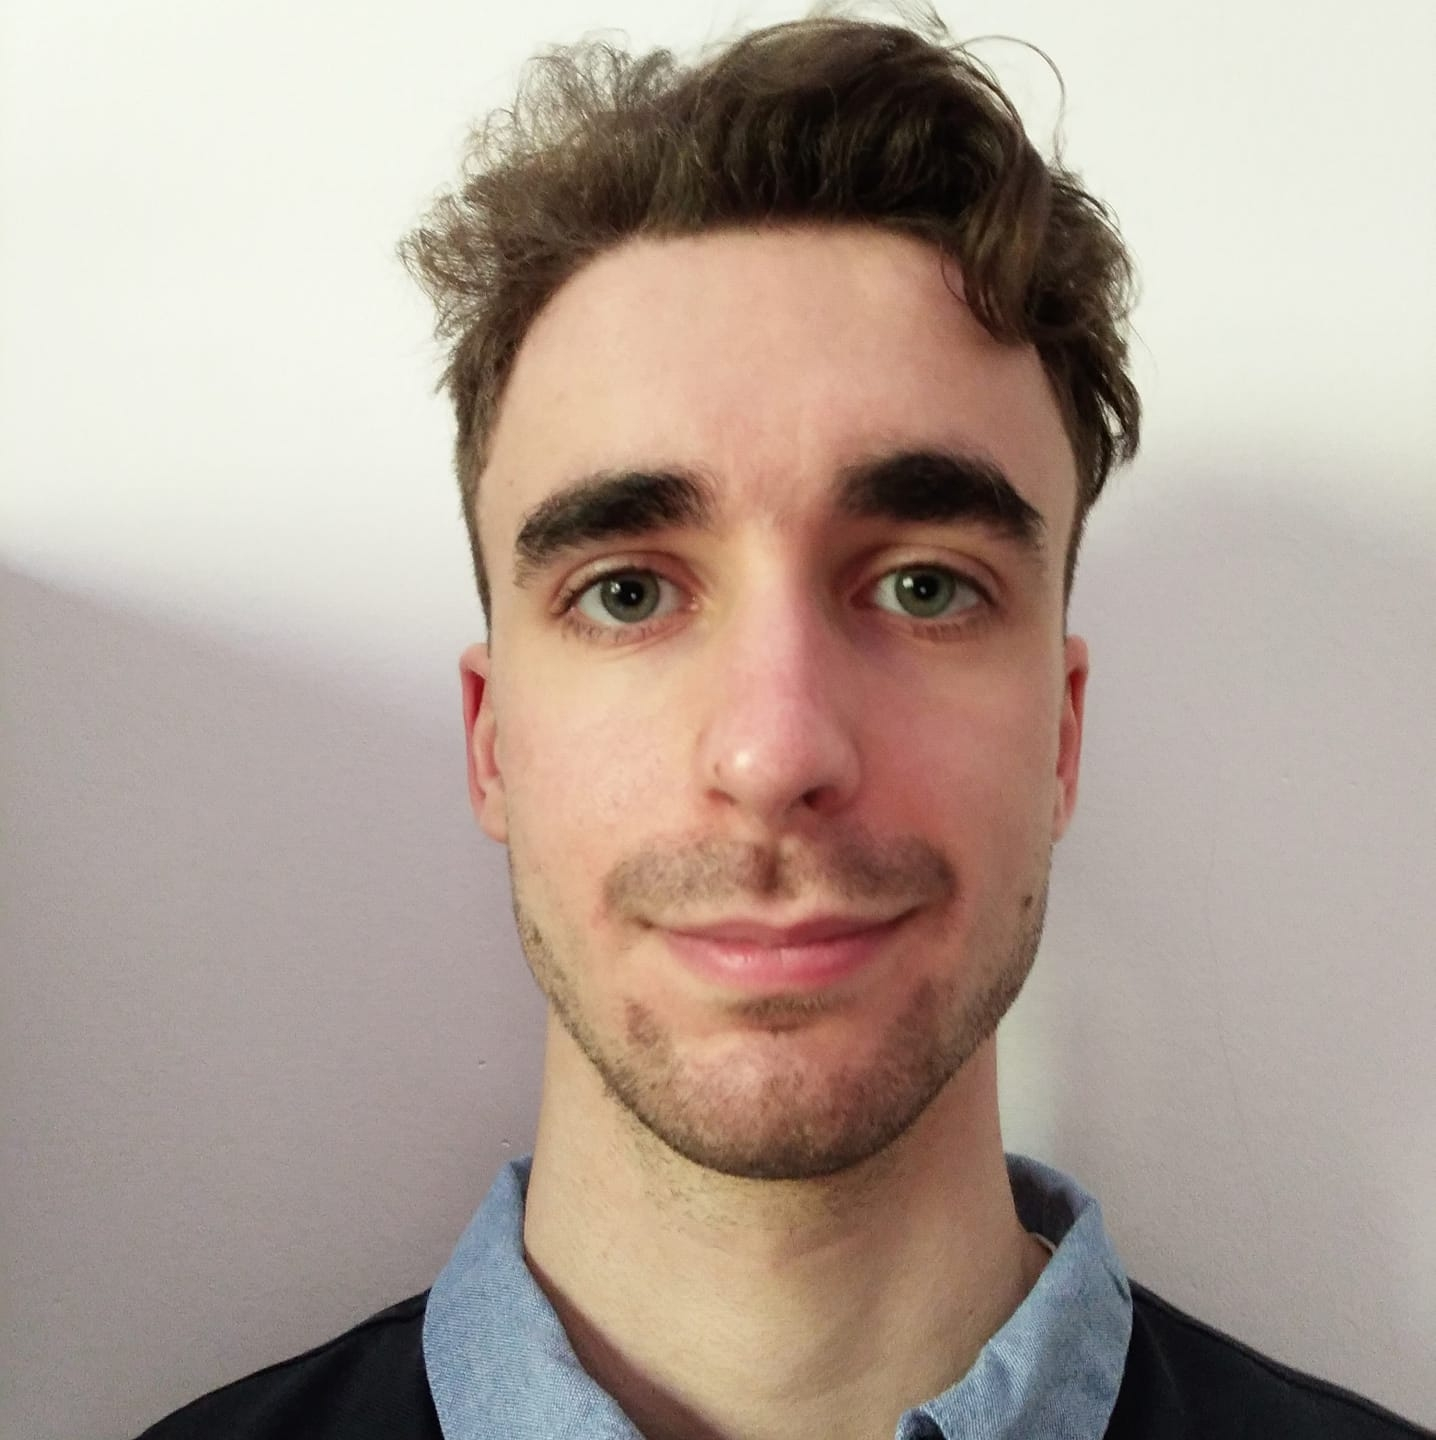
\includegraphics[width=3.7cm]{Matteo.jpg}\par}	%trimming relative to image size

    %\vfill\null
    \cvsection{CONTACT}

    \icontext{MapMarker}{12}{Via Campolino, 35\\35010 Vigonza(PD)}{black}\\[6pt]
    \icontext{MobilePhone}{12}{+39 347 381 83 58}{black}\\[6pt]
    \iconemail{Envelope}{12}{matteo.marchiori97@gmail.com}{matteo.marchiori97@gmail.com}{black}\\[6pt]

    %\vfill\null
    \cvqrcode{0.5}

    %---------------------------------------------------------------------------------------
    %	META SKILLS
    %----------------------------------------------------------------------------------------
    \cvsection{SKILLS}

    \cvskill{Python} {} {1} \\[-2pt]
    \cvskill{Scrapy} {} {1} \\[-2pt]
    \cvskill{Flutter} {} {.7} \\[-2pt]
    \cvskill{Angular} {} {.8} \\[-2pt]
    \cvskill{PHP, JS, CSS, HTML} {} {1} \\[-2pt]
    \cvskill{Bootstrap, JQuery} {} {1} \\[-2pt]
    \cvskill{Ecommerce CMS} {} {1} \\[-2pt]
    \cvskill{Apache2, Nginx} {} {1} \\[-2pt]
    \cvskill{Postfix, Dovecot} {} {1} \\[-2pt]
    \cvskill{Java, C++} {} {.8} \\[-2pt]
    \cvskill{Spring} {} {.8} \\[-2pt]
    \cvskill{R} {} {.6} \\[-2pt]
    \cvskill{CI/CD tools} {} {.6} \\[-2pt]
    \cvskill{LaTeX} {} {.6} \\[-2pt]
    \cvskill{XML, JSON} {} {1} \\[-2pt]
    \cvskill{MySQL, MongoDB} {} {1} \\[-2pt]
    \cvskill{Windows \& Linux} {} {1} \\[-2pt]
    \cvskill{Office} {} {1} \\[-2pt]

    %---------------------------------------------------------------------------------------
    %	EDUCATION
    %----------------------------------------------------------------------------------------
    \newpage
    \cvsection{EDUCATION}

    \cvmetaevent
    {2019 - today}
    {M. Sc. Computer Science}
    {University of Padua}
    {
        \begin{itemize}
            \item IT Service Management
            \item Information Retrieval 
            \item Mobile programming and Multimedia
            \item Wireless Networks
            \item Data Mining
            \item Formal methods for Cyberphysical systems
            \item Computer and Network security
            \item Advanced algorithms
            \item Innovation economy
            \newline
        \end{itemize}
    }

    \cvmetaevent
    {2016 - 2019}
    {B. Sc. Computer Science (102/110)}
    {University of Padua}
    {
        \begin{itemize}
            \item Thesis: Migration of a Web application with monolithic architecture towards a microservices architecture
            \item Software Engineering
            \item Web technologies
            \item Open source technologies
            \item Network and security
            \item Databases
            \item Object Oriented Programming
            \item Concurrent and distributed programming
            \newline
        \end{itemize}
    }

    \newpage
    \cvmetaevent
    {2011 - 2016}
    {IT High school diploma (98/100)}
    {ITIS F. Severi, Padua}
    {
        \begin{itemize}
            \item School projects for network administration
            \item Networks and protocols (DNS, HTTP, etc.)
            \item Back-end and front-end languages for Web development
            \item Database administration
            \item OOP languages
            \item Android apps development
            \newline
        \end{itemize}
    }

    %\vfill\null
    %\cvqrcode{0.7}

    %---------------------------------------------------------------------------------------
    %	CERTIFICATION
    %----------------------------------------------------------------------------------------
    \cvsection{CERTIFICATIONS}

    \cvmetaevent
    {Cambridge ESOL - B2}
    {}
    {}
    {
        \begin{itemize}
            \item Overall score 179/210
            \item Reading 177/210
            \item Use of English 193/210
            \item Writing 177/210
            \item Listening 169/210
            \item Speaking 181/210
        \end{itemize}
    }

    %\vfill
    %\cvqrcode{0.7}

    %\newpage
    %\mbox{} % hotfix to place qrcode on the bottom when there are not other elements
    %\vfill
    %\cvqrcode{0.7}

\end{leftcolumn}
\begin{rightcolumn}
%---------------------------------------------------------------------------------------
%	TITLE  HEADER
%----------------------------------------------------------------------------------------
\fcolorbox{white}{darkcol}{\begin{minipage}[c][3.5cm][c]{1\mpwidth}
    \begin {center}
    \HUGE{ \textbf{ \textcolor{white}{ Matteo Marchiori } } } \\[-24pt]
    \textcolor{white}{ \rule{0.1\textwidth}{1.25pt} } \\[4pt]
    \large{ \textcolor{white} {Full Stack Developer} }
    \end {center}
    \end{minipage}} \\[14pt]
\vspace{-12pt}

%---------------------------------------------------------------------------------------
%	PROFILE
%----------------------------------------------------------------------------------------
\vfill\null
\cvsection{PROFILE}

\cvtext{Passioned about IT since always.\\

    Currently working as a full stack developer for monolithic Web platforms, websites and ecommerce.\\

    My focus is on how technology can solve higher problems, and on how many resources need to be employed to get the agreed service level.\\

}

%---------------------------------------------------------------------------------------
%	WORK EXPERIENCE
%----------------------------------------------------------------------------------------
\vfill\null
\cvsection{WORK EXPERIENCE}

\cvevent
{2016 - today}
{DevOps/FullStack developer}
{Research and Development}
{Working for DAVID MONETTI s.r.l. with the main focus on managing servers, websites and emails.}
{\cvlist{
        \item Web server management
        \item Email server management 
        \item Website creation (Wordpress, Woocommerce, Opencart, pure PHP + JavaScript + CSS + HTML, Bootstrap)
        \item Data analysis
    }}
{\cvlist {
        \item Amazon EC2
        \item Wordpress
        \item Woocommerce
        \item Opencart
        \item PHP/JavaScript/CSS/HTML
        \item Bootstrap
        \item Google Search Console
        \item Google Analytics
    }}
{\cvlist{
        \item Websites and ecommerce
        \item Improvements on SEO and security of websites
        \item Improvements on communication and team working
    }}

\vfill\null
\cvevent
{09/2020 - 11/2020}
{App development}
{Research and Development}
{Development of a Flutter app for a friend.}
{\cvlist{
        \item Mobile development
    }}
{\cvlist {
        \item Flutter
    }}
{\cvlist{
        \item App to manage Amazon deliveries from a third party customer
    }}

\vfill\null
\cvevent
{2019 - 2020}
{IT manager}
{Management}
{Responsible for IT with some friends for WEB TOP ADAPTIVE AI s.r.l.}
{\cvlist{
        \item Resource management
        \item Platform management
        \item Website management
    }}
{\cvlist {
        \item PHP/JavaScript/CSS/HTML for the Web application
        \item Python for client side application
    }}
{\cvlist{
        \item Bot for Instagram
        \item Improvement on resource asset planning and management
    }}

\vfill\null
\cvevent
{06/2018 - 10/2018}
{Web app developer}
{Web Development}
{Contributes for a project for Gruppo Fondiario Italia s.r.l. for a Web application.}
{\cvlist{
        \item Web application to check costs and advantages of energy efficiency interventions on buildings
    }}
{\cvlist {
        \item PHP/JavaScript/CSS/HTML
        \item Bootstrap
    }}
{\cvlist{
        \item Web application
    }}

\vfill\null
\cvevent
{02/2018 - 04/2018}
{Scraper developer}
{Web development}
{Contributes for a project for WARDA s.r.l. for scrapers on luxury brands.}
{\cvlist{
        \item scrapers for ecommerce websites
    }}
{\cvlist {
        \item Scrapy
        \item Python
    }}
{\cvlist{
        \item Scrapers for websites
    }}

\vfill\null
\cvevent
{07/2015 - 08/2015}
{Java application}
{Stage}
{Application to check the energy efficiency of a building}
{\cvlist{
        \item Static application to check the energy efficiency based on some papers values
    }}
{\cvlist {
        \item Java
    }}
{\cvlist{
        \item Some useful graphs
    }}

%\vfill\null
%\cvevent
%{06/2015 - 07/2015}
%{PC formatting}
%{Technical department}
%{Formatting of some pcs at NED training center in Dublin.}
%{\cvlist{
%        \item PC formattig with Linux and Windows
%        \item PC assembly
%        \item Network administration
%    }}
%{\cvlist {
%        \item Windows/Linux
%    }}
%{\cvlist{
%        \item Three working pcs from five not working
%    }}


%---------------------------------------------------------------------------------------
%	COMMUNICATION SKILLS
%----------------------------------------------------------------------------------------
\vfill\null
\cvsection{COMMUNICATION SKILLS}

\cvtext{
    \begin{itemize}
        \item team working with a communication agency
        \item team working with my work mates at WEB TOP ADAPTIVE AI
        \item project for Software Engineering with other five people
    \end{itemize}
}

%---------------------------------------------------------------------------------------
%	PERSONAL DATA
%----------------------------------------------------------------------------------------
\vfill\null
\cvsection{PERSONAL DATA}

\cvtext{
    I hereby authorize the use of my personal data in accordance to the GDPR 679/16 - ``European regulation on the protection of personal data''.
}

% hotfixes to create fake-space to ensure the whole height is used
\mbox{}
\vfill
\mbox{}
\vfill
\mbox{}
\vfill
\mbox{}
\end{rightcolumn}
\end{paracol}
\end{document}

